\section{System Design}
The core idea of the \textit{Mobility Feature Package} is to provide a very simple programming interface such that computing features can be done with very few lines of code. This requires closing of the internal working of the package off, such that the programmer has very limited ways in which he/she can interface with it. The design of the package API went through two main iterations which consisted of many smaller iterations. Mainly, the difference between the final iteration and the earlier iterations is the amount of code required for managing historical data that the programmer has to write. Early iterations put the responsibility on the application programmer to manage historical data. After developing the field study app discussed in chapter \ref{chapter:06} it was decided to move most of this logic inside the package; it became glaringly apparent that the package was too cumbersome to use. The final iteration is the one discussed in this thesis including the choices and lessons learned on the way of designing and developing it. 


\subsection{Component Overview}
Figure \ref{fig:component-diagram-internal} displays how the final iteration looks like as a software system: The main component is the \textit{Context Generator} component which is the interface that the programmer will use. This component exposes two interfaces to the programmer allowing the user to store their collected \textit{LocationSamples} as well as generate a \textit{Mobility Context} that contains the daily features. The two exposed interfaces are provided by the programmer through mobile application. The \textit{Context Generator} is also responsible for storing and loading data via the \textit{Mobility Serializer} component, here the \textit{Serializable} type refers to any data type that needs to be stored as historical data.

\begin{figure}[h]
\centering
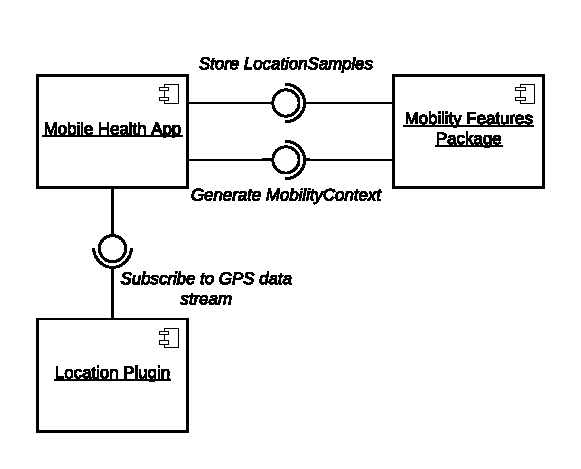
\includegraphics[width=\textwidth]{images/diagrams/component-external.pdf}
\caption{Component diagram for the \textit{Mobility Feature Package} from an internal point of view}
\label{fig:component-diagram-internal}
\end{figure}

Figure \ref{fig:component-diagram-external} shows the external software system that includes the mobile application using the package. Another design choice is reflected in this figure which is the usage of an external location plugin which must be done by the programmer. This means task the programmer has to collect their own location data through their location plugin which will collect location \textit{Data Transfer Objects} (DTOs) \cite{fowler-PEEA} [p. 401]. These objects hold location data, i.e. latitude, longitude, and a timestamp and can be converted to \textit{LocationSamples} and saved through the \textit{Mobility Feature Package.}
Two reasons led to this decision, the first of which being that the Mobility Features Package becomes more loosely coupled and modular. The second reason relates to maintenance; if the package was to implement location data collection then it becomes harder to maintain since any change to the location plugin would imply changes to the Mobility Features Package as well. 

\begin{figure}[h]
\centering
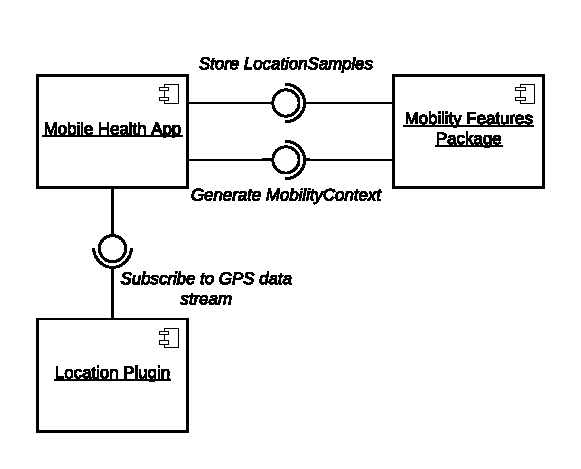
\includegraphics[width=\textwidth]{images/diagrams/component-external.pdf}
\caption{Component diagram for the \textit{Mobility Feature Package} from an internal point of view}
\label{fig:component-diagram-external}
\end{figure}


\subsection{Sequence Overview}
To display the interactions between the components, sequence diagrams are used. Figure \ref{fig:sequence-diagram-external} shows the system from an external point of view, where the application subscribes to location updates via the location plugin, saves location data via the Mobility Features Package and generates a Mobility Context through it. 

\begin{figure}[h]
\centering
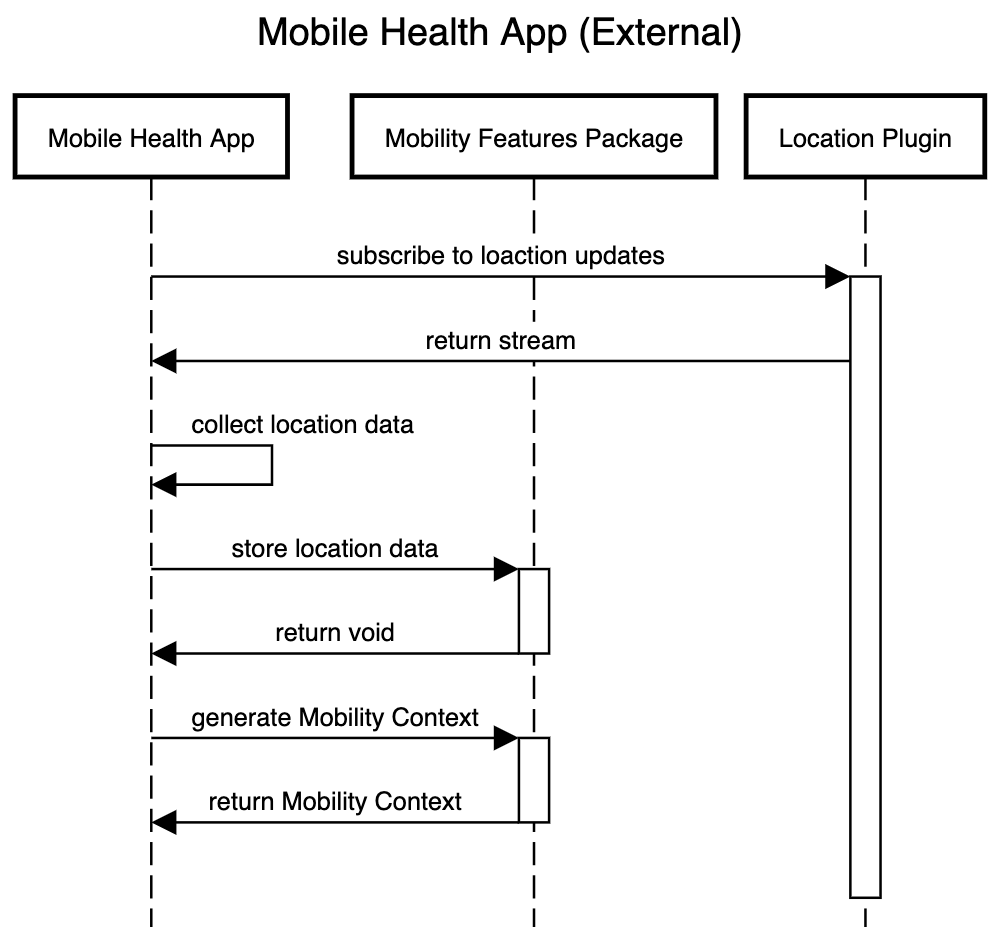
\includegraphics[width=\textwidth]{images/diagrams/sequence-external.png}
\caption{Component diagram for the \textit{Mobility Feature Package} from an internal point of view}
\label{fig:sequence-diagram-internal}
\end{figure}

From an internal point of view, the \textit{Context Generator} component calls the \textit{Mobility Serializer} for storing and loading historical data, uses the loaded data to generate a \textit{Mobility Context} by calling the MobilityContext component.
\begin{figure}[h]
\centering
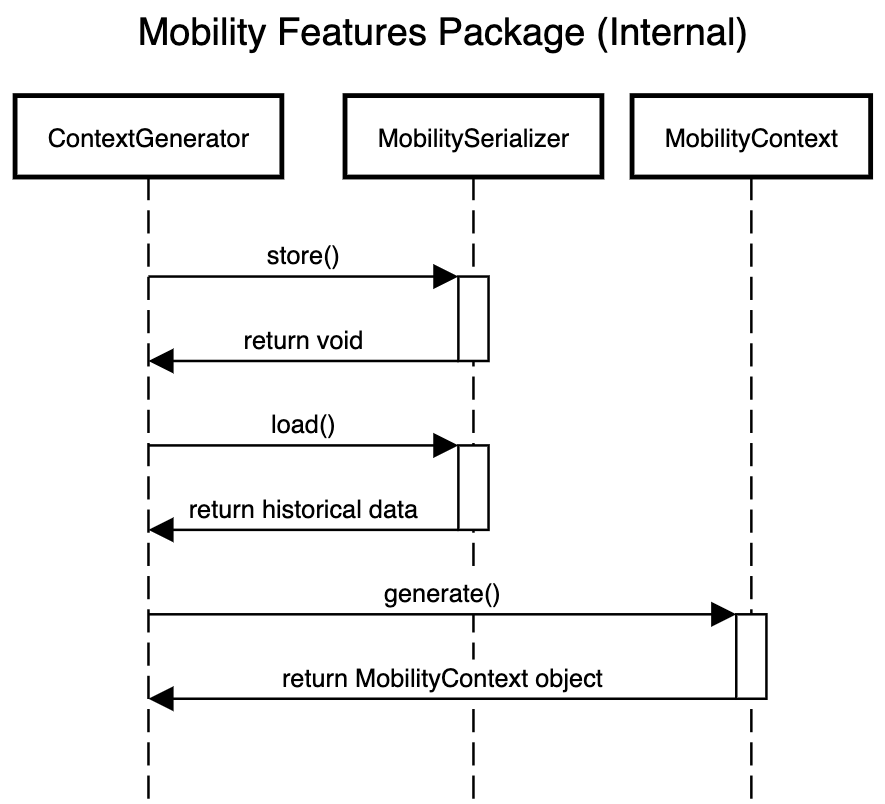
\includegraphics[width=\textwidth]{images/diagrams/sequence-internal.png}
\caption{Sequence diagram for mobile health application using the Mobility Features Package, i.e. viewed externally from the package}
\label{fig:sequence-diagram-external}
\end{figure}